\documentclass[a4paper,8pt,oneside]{article}

\usepackage{pgfplots}
\usepackage{amsmath}

% \titleformat{\section}{\normalfont\fontsize{10}{10}\bfseries}{\thesection}{1em}{}

\author{Luca Zamboni}
\title{\vspace{-4em} \LARGE First Project - Report}
\date{\today}

\begin{document}

% \maketitle

% GOOD Report that includes: Data Analysis
% Evaluation
% Comparison of different:
% Feature Sets
% Tool Configurations

\begin{titlepage}
	\pagestyle{empty}

	\begin{center}
		{\bfseries\Large {\huge U}NIVERSITY OF {\huge T}RENTO}

		\vspace{0.2cm}

		{\large Department of Information Engineering and Computer Science}

		\vspace{5.5cm}

		{\Large \bfseries {{\huge L}ANGUAGE {\huge U}NDERSTANDING} {\huge S}YSTEM}

		\vspace{1.0cm}

		{\Large \bfseries {FIRST PROJECT}}

		\vspace{2.5cm}
		
		{\large \textsc{Zamboni Luca}}

		\vspace{1.0cm}
		
		{\today}

		\vfill

	\end{center}

\end{titlepage}


\tableofcontents
\newpage
\section{Sequence lebeling}

	In this section will be analyzed and discussed the performance 2 different methods for the sequence lebeling task. Final state transducer (FST) based on POS-Tagging and Conditional random fields (CRF) based on IOB notation.

	\subsection{FST}
		\subsubsection{Data analysis}
			The training set and the test set are composed with 3 columns: token POS-tag lemma.
			The token is a word of the sentence with his relative POS-tag and his lemma. Every sentence is separated with a empty line. Token are 21453 for a total of 3337 sentences. Lemmas are a generalization of the relative words. For example the plural and the singular of a given word have the same lemma. The distribution of POS-tags among the dataset is described in Figure \ref{tag-dist}. As we can see POS-tags are not equally distributed and there are few tags that take almost all probability.
			\begin{figure}[h!]
			  \centering
			    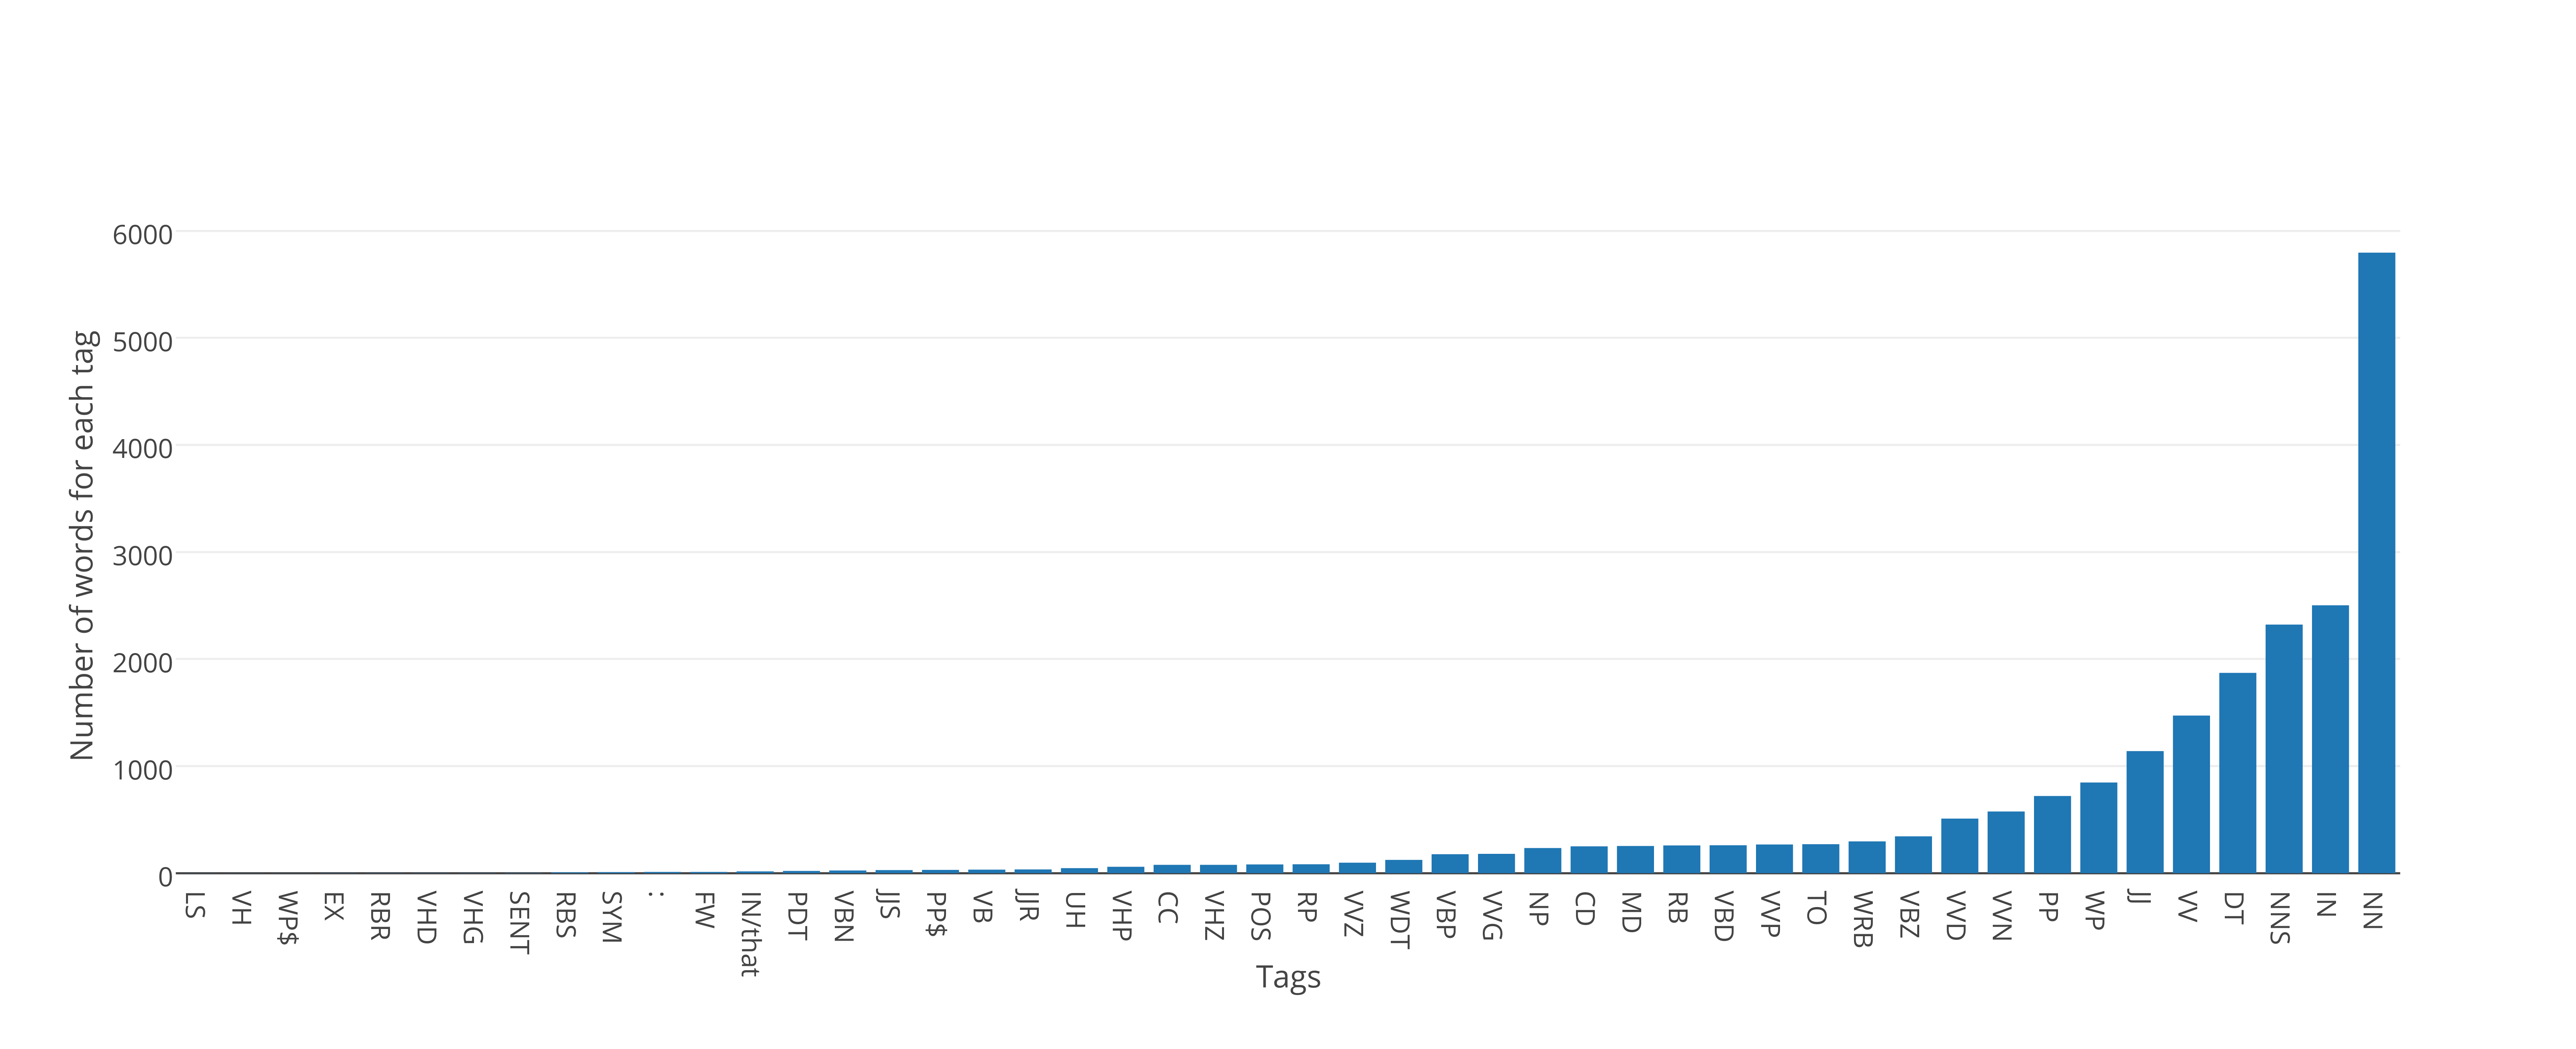
\includegraphics[width=1.0\textwidth]{img/barcharttag}
			  \caption{Bar chart of the distribution of number of words for each tag.}
			  \label{tag-dist}
			\end{figure}
		\subsubsection{Tools}
			The tools used for the train and test:
			\begin{itemize}
				\item OpenFst used to create and compose fsts for unigram
				\item OpenNgr used to automatically train models with n-grams
			\end{itemize}
		\subsubsection{Training}
			First of all i created a file with the following structure
			\begin{equation}
				word \qquad tag \qquad -log(P(w_i|t_i)))
			\end{equation}
			Where $P(w_i|t_i)$ is the probability of a word given a tag and is computed with the following formula $\frac{C(w_i,t_i)}{C(t_i)}$. $C(w_i,t_i)$ is the count of the word with a particular tag and $C(t_i)$ is the numer of appearance of a tag in the training test. I used minus log of the probability because in this way higer probability take a lower number than minus log of a  a low probability and this will be needed later. Then i created the transducer for the model in the following way:
			\begin{gather*}
					0 \qquad 0 \qquad word \qquad tag \qquad -log(P(w_i|t_i)) \\
					... \\
					0 \qquad 0 \qquad word \qquad tag \qquad -log(P(w_i|t_i)) \\
			\end{gather*}
			This transducer is our model based on unigrams. Now we want consider also the probability of a tag given the predecessor. To do this i used the Opne-ngr tool that automatically creates the model of n-grams of token. The command that i used are the following:\\ \\

			\textbf{farcompilestrings} --unknown\_symbol='$<$unk$>$' input.txt $>$ far.far \\
			\textbf{ngramcount} --order=N --require\_symbols=false far.far $>$ input.cnt \\
			\textbf{ngrammake} --method=witten\_bell input.cnt $>$ ngrammodel.lm \\ \\

			Where the paramether of the 
			The final output is a fst that rappresent out model of 3-gram POS-tag.
			Now that i trained my model i can test it.

		\subsubsection{How to test}
		    To test a sentence i created a fst for each sentence in this way:
			\begin{gather*}
					0 \quad 1 \quad word1 \quad word1 \\
					1 \quad 2 \quad word2 \quad word2 \\
					... \\
					(N-1) \quad N \quad wordN \quad wordN	
			\end{gather*}
			Now this fst is composed with the fst that represent our unigram-tag model. \\ \\
			\textbf{fstcompose} input-sentence.fst unigram-model.fst $>$ word-tagged-unigram.fst \\ \\
			Now we have a simple tagger based on unigrams. To use also the model based on n-gram of tags we just compose the previous tagger with this. \\ \\
			\textbf{fstcompose} simple-tagger.fst n-gram-model.fst $>$ word-tagged-n-gram.fst \\ \\
			And after to get the best tagger we just run the command fstshortestpath. We can use the command shortest path because is not the real probability but the minus log o probability and in this way with this command we get the most probable sequence of tag. All command togheter in order to get a sequance of POS-tag of a sentence: \\ \\
			\textbf{fstcompose} input-sentence.fst unigram-model.fst $>$ word-tagged-unigram.fst \\
			\textbf{fstcompose} simple-tagger.fst n-gram-model.fst $>$ word-tagged-n-gram.fst \\
			\textbf{fstrmepsilon} word-tagged-n-gram.fst $|$ fstshortestpath $>$ final-tag.fst \\ \\

			The result is a fst that take as input a sentence and gives the best possible sequence of POS-tag like the one in Figure \ref{tagger-final}
			\begin{figure}[h!]
			  \centering
			    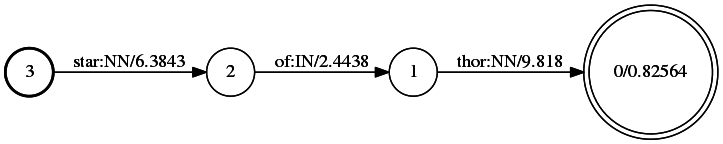
\includegraphics[width=1.0\textwidth]{img/tagger}
			  \caption{Final result of POS-tagger}
			  \label{tagger-final}
			\end{figure}
		\subsubsection{Results of testing}
			The test set is structured in the same way of the training set. This set has 7117 words each with the expected POS-tag. First i runned the test set with a simple tagger without n-grams of tag and after with. I also runned a train and test with lemmas. To evaluate the test was used a script in perl conneval.pl.
			\begin{table}[h]
				\begin{tabular}{ccccc}
					& \textbf{Accuracy} & \textbf{Precision} & \textbf{Recall} & \textbf{F1 Score} \\
					\textbf{Unigram word POS-tag} & 84.91\%           & 83.20\%            & 84.61\%         & 83.90 \\
					\textbf{2-gram POS-tag}       & 93.37\%           & 91.98\%            & 92.45\%         & 92.77 \\
					\textbf{3-gram POS-tag}       & 93.80\%           & 92.51\%            & 93.04\%         & 92.77 \\
					\textbf{3-gram POS-tag with lemma}       & 78.22\%           & 75.80\%            & 74.09\%         & 74.94 \\
				\end{tabular}
				\caption{Result of test}
			\end{table}
			accuracy:  94.13%; precision:  92.87%; recall:  93.29%; FB1:  93.08

			The best result is in the model based on 3-gram. As we can see in the table, the simple POS-tagger is less precise of the tagger based on n-gram. This because using we do not consider only probability as word but also the previous word and the previous tag. As we can se from the table if we train our model considering also the lemma accuracy goes down a lot this because maybe inenghlish lemma doesn't cont too much.Perhaps they can be useful in other language like Italian where the grammar is more complex. We can conclude that the model based on 3-gram is the best for accuracy. The model based on 4-gram is too complex and it risk to fit also the rumor of data do i decided to do not consider that.

	\subsection{CRF}
		\subsubsection{Data analysis}
			The training set is composed with 2 column: one for the token and the other with the relative tags in IOB-notation. Words are 21453 for a total of 3338 phrases. The distribution of the tags is described in the Figure \ref{crf-dist}.
			\begin{figure}[h!]
			  \centering
			    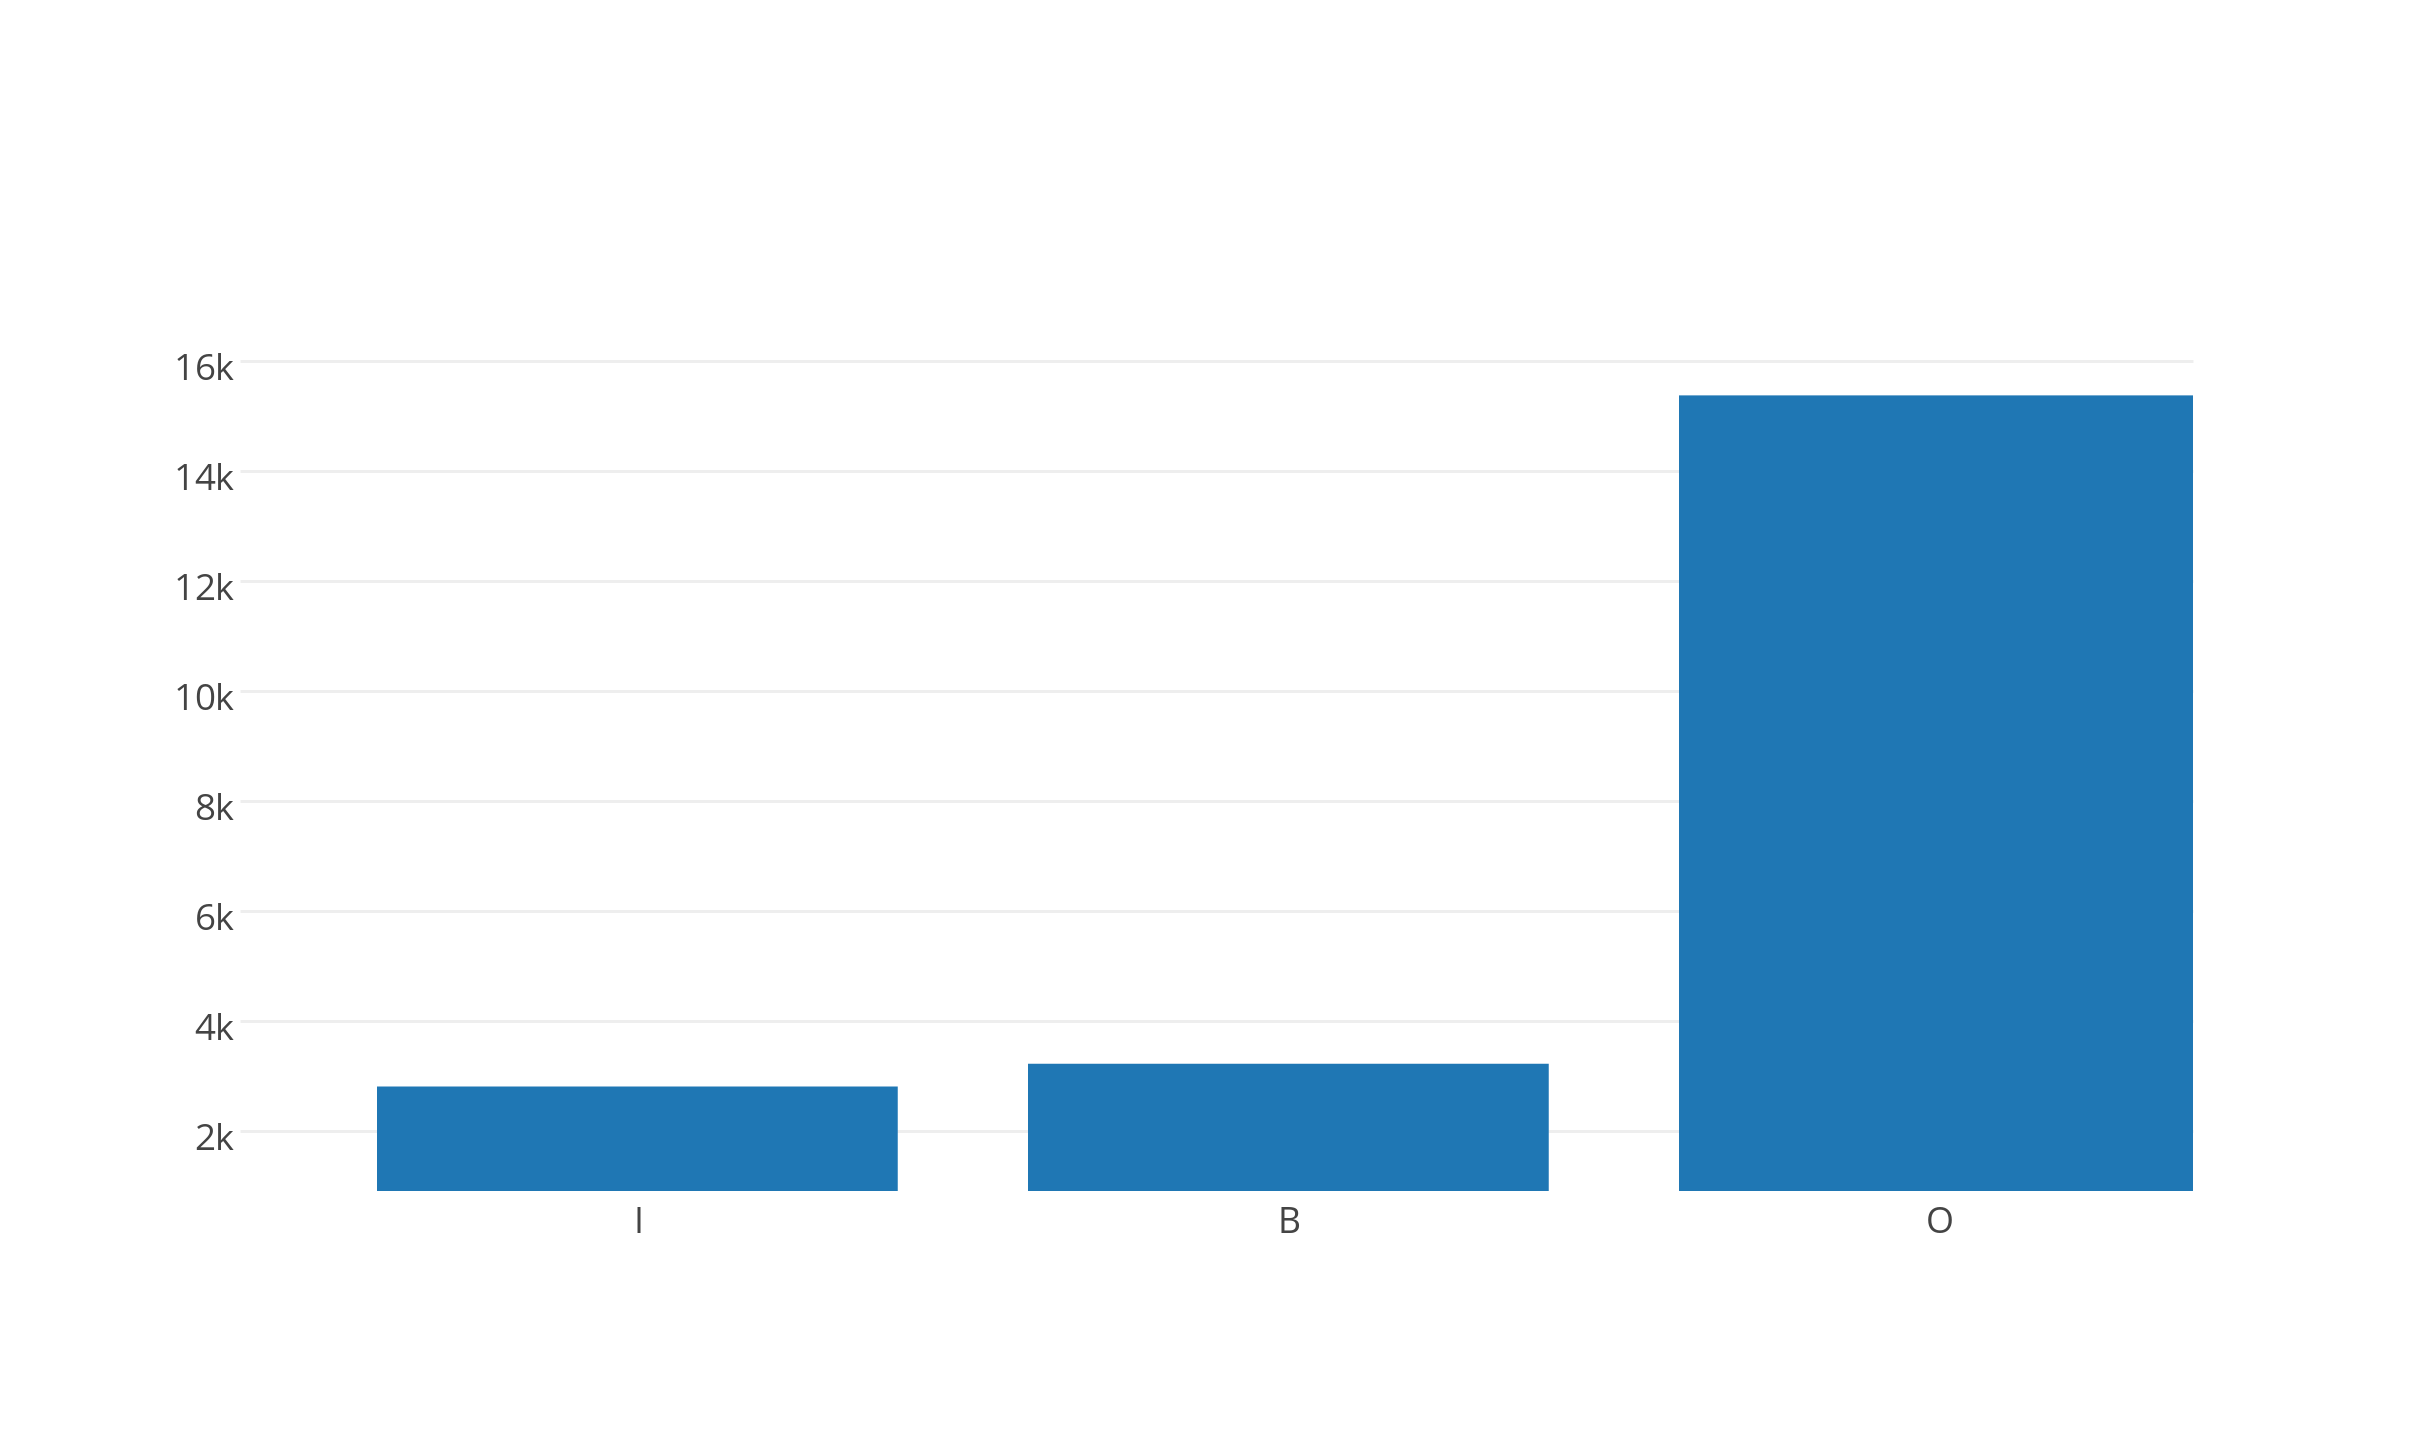
\includegraphics[width=1.0\textwidth]{img/crf-dist}
			  \caption{Distribution of I O B.}
			  \label{crf-dist}
			\end{figure}
		\subsubsection{Tool}
			The tools used for the train id CRF++. It is a tollkit to automatically train and test conditional random fields.
		\subsubsection{Training}
			To train with this tool we need a template for feature extracting.
			An example of template is: \\ \\
			U01:\%x[-1,0] \\
			U02:\%x[0,0] \\
			U03:\%x[1,0] \\ \\
			Whit this template you consider 3 words at time as feature. \\
			The command to train is \\\\
			\textbf{crf\_learn} template\_file train\_file model\_file\\\\
			The model\_file is our trained model in output.
		\subsubsection{Testing}
			To test we must simply run the command \\ \\
			\textbf{crf\_test} -m model\_file test\_files \\ \\
			It outputs a file with token, expected tag and tag predicted by the model. After that to calculate statistics i used a perl file conneval.pl that calculate automatically: accuracy, precision, recall and F1 score. I runned different train with different template file and result are described in the following table with relative template below.
			\begin{table}[h]
				\centering
				\begin{tabular}{ccccc}
					& \textbf{Accuracy} & \textbf{Precision} & \textbf{Recall}  & \textbf{F1 Score} \\
					\textbf{Template 1} & 87.59\%  & 44.99\%   & 60.49\% & 51.60    \\
					\textbf{Template 2} & 92.38\%  & 65.98\%   & 67.55\% & 66.7     \\
					\textbf{Template 3} & 93.76\%  & 76.97\%   & 74.43\% & 75.68    \\
					\textbf{Template 4} & 94.23\%  & 86.35\%   & 78.28\% & 82.12    \\
				\end{tabular}
				\caption{Result of test}

			\end{table}
			\begin{table}[h]
				\begin{tabular}{llll}
					\begin{tabular}[c]{@{}l@{}}U02:\%x{[}0,0{]}\\ \\ \\ \\ \\ \\ \\ \\ \\ \\ \\ \\ \\ \textbf{Template 1}\end{tabular} & \begin{tabular}[c]{@{}l@{}}U00:\%x{[}-2,0{]}\\ U01:\%x{[}-1,0{]}\\ U02:\%x{[}0,0{]}\\ U03:\%x{[}1,0{]}\\ U04:\%x{[}2,0{]}\\ \\ \\ \\ \\ \\ \\ \\ \\ \textbf{Template 2}\end{tabular} & \begin{tabular}[c]{@{}l@{}}U00:\%x{[}-2,0{]}\\ U01:\%x{[}-1,0{]}\\ U02:\%x{[}0,0{]}\\ U03:\%x{[}1,0{]}\\ U04:\%x{[}2,0{]}\\ U05:\%x{[}-1,0{]}/\%x{[}0,0{]}\\ U06:\%x{[}0,0{]}/\%x{[}1,0{]}\\ \\ \\ \\ \\        \\ \\ \textbf{Template 3}\end{tabular} & \begin{tabular}[c]{@{}l@{}}U00:\%x{[}-2,0{]}\\ U01:\%x{[}-1,0{]}\\ U02:\%x{[}0,0{]}\\ U03:\%x{[}1,0{]}\\ U04:\%x{[}2,0{]}\\ U05:\%x{[}-1,0{]}/\%x{[}0,0{]}\\ U06:\%x{[}0,0{]}/\%x{[}1,0{]}\\ B00:\%x{[}-2,0{]}\\ B01:\%x{[}-1,0{]}\\ B02:\%x{[}0,0{]}\\ B03:\%x{[}1,0{]}\\ B04:\%x{[}2,0{]}\\ \\ \textbf{Template 4}\end{tabular}
				\end{tabular}
			\end{table}
			As we can see from the tables template 4 is the one with higher performance.
			Template 1 and 2 are very semple and they have a very little window. Template 3 and 4 have a template more complex and they have a similar accuracy but Template 4 have a greater F1 Score. In conclusion i can say that template 4 is the one with best performance because it is more complex because it consider also bigrams.
\section{Text classification}
	\subsection{Naive Bayes}
		\subsubsection{Goal}
			Train a model with sentences and relative tag in order to output a tag given a sentence.
		\subsubsection{Data analysis}
			The training set is composed by sencences with relative tag. Sencences are 3338.
			The distribution of tags is described in Figure \ref{bayes-dist}. As we can see movie is the tags with more probability.
			\begin{figure}[h!]
			  \centering
			    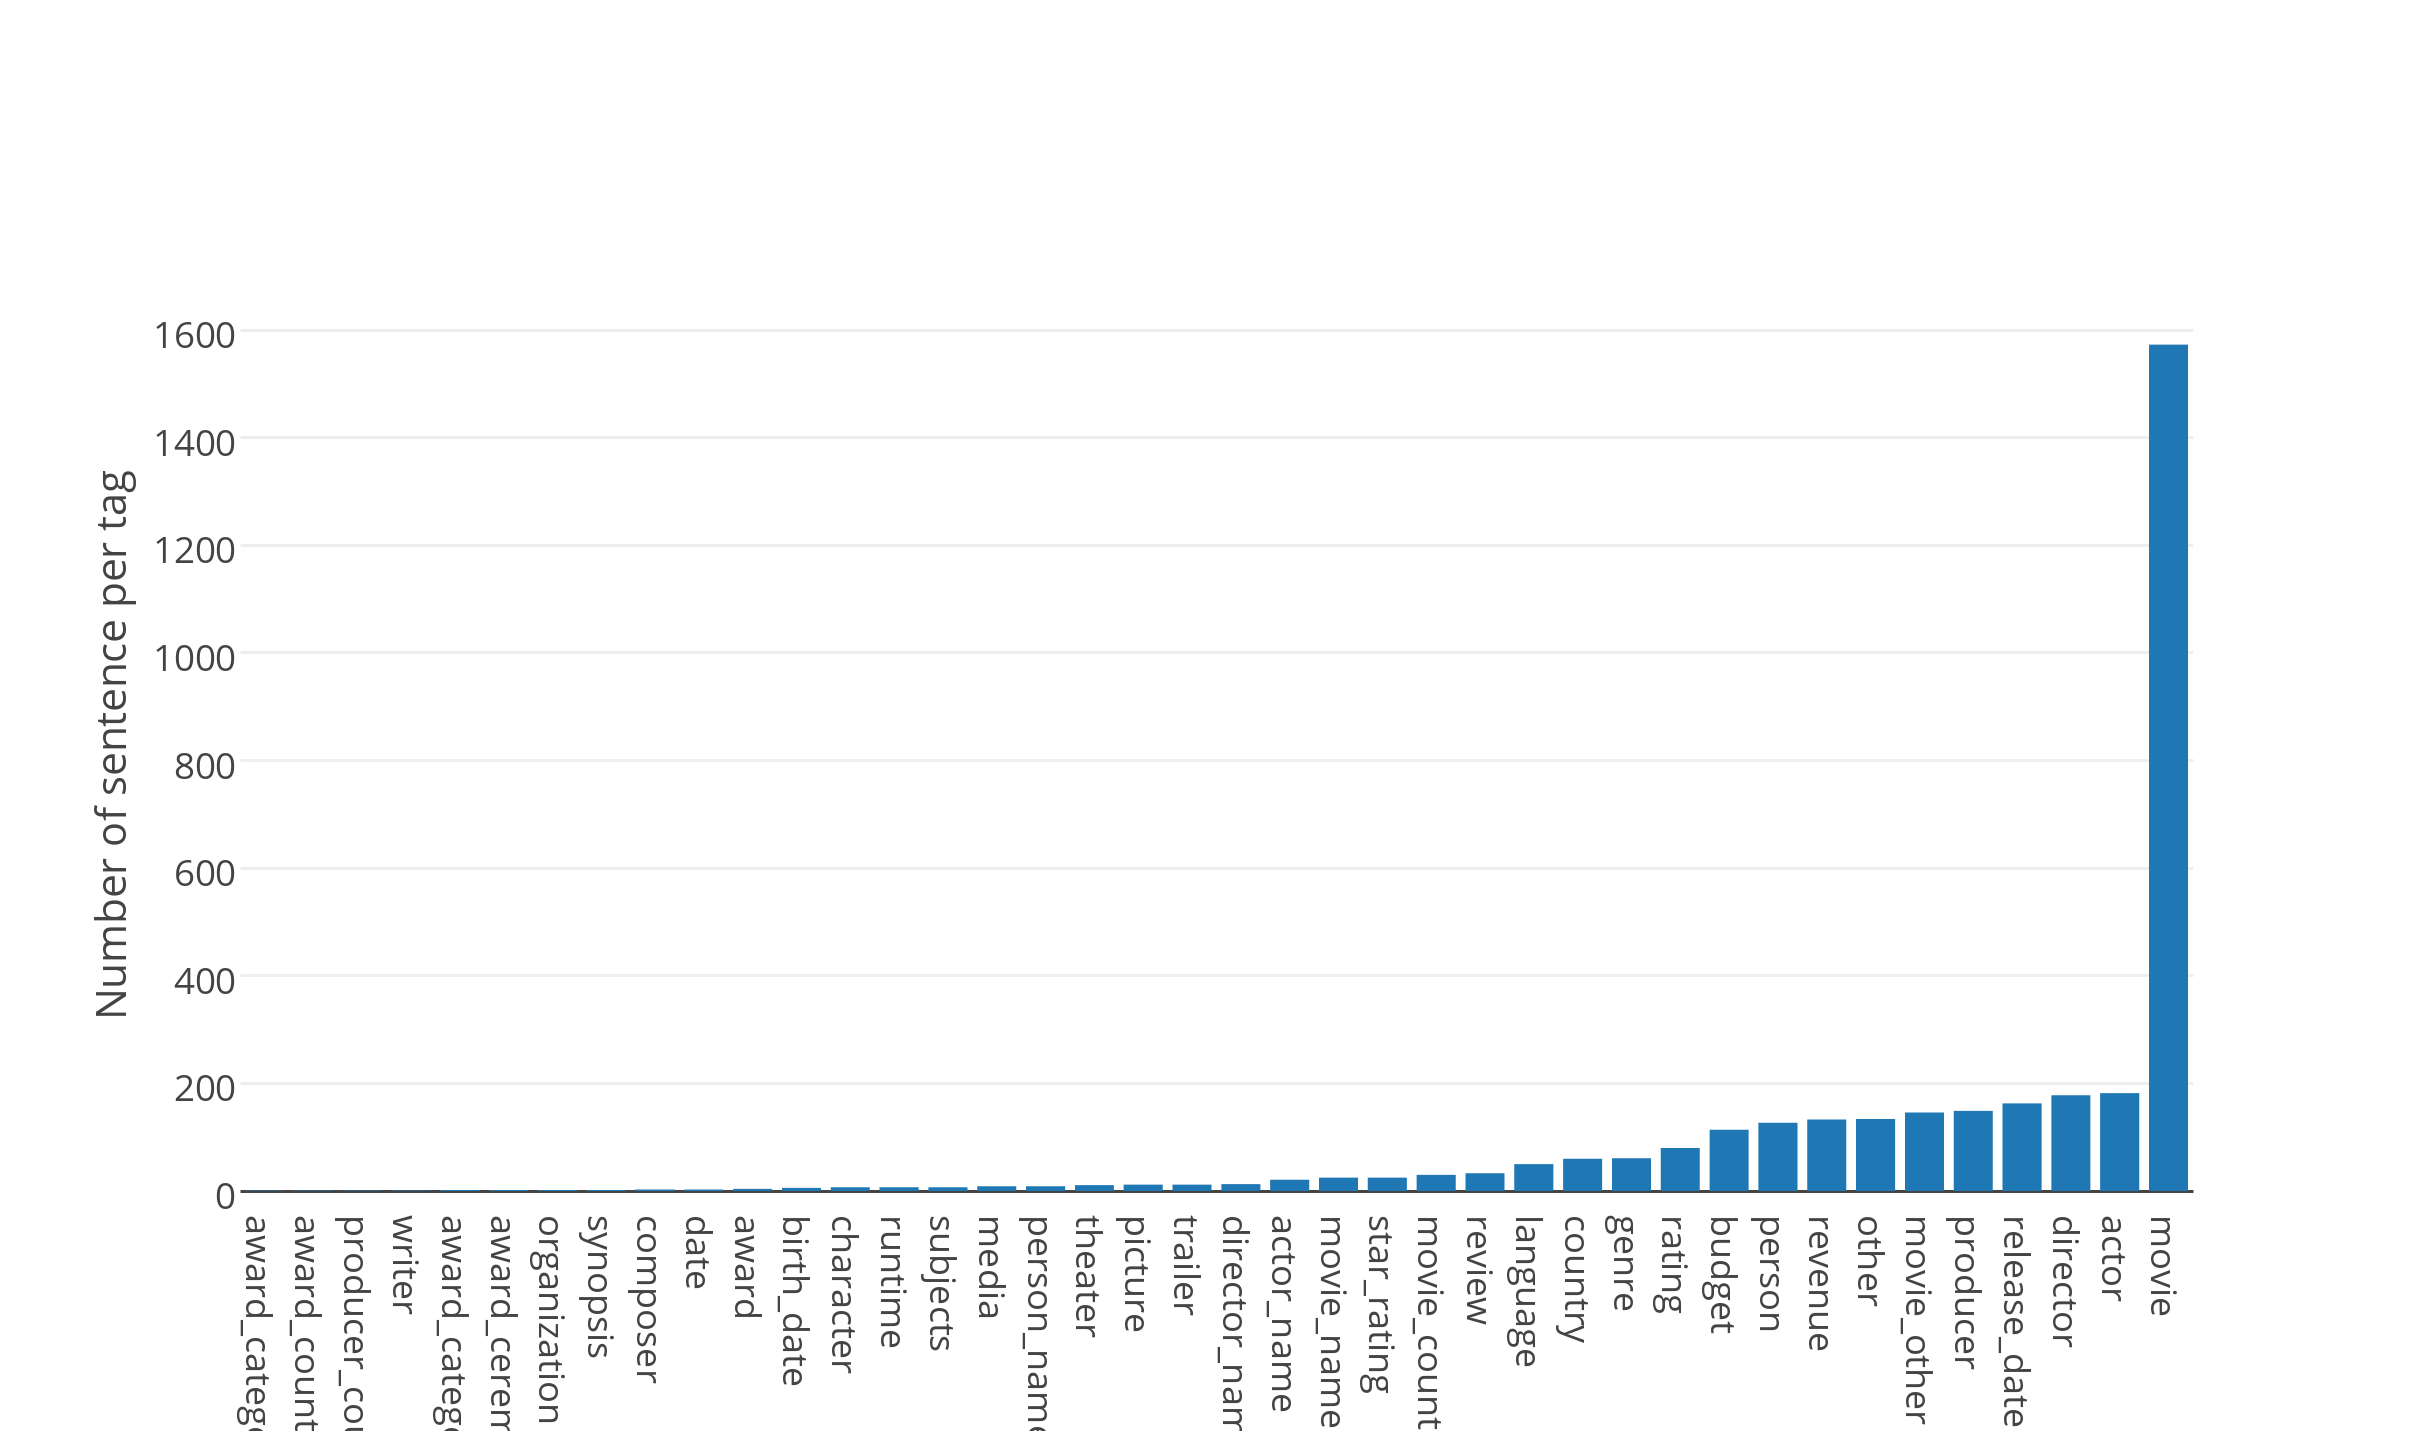
\includegraphics[width=1.0\textwidth]{img/bayes-tag}
			  \caption{Distribution of tags.}
			  \label{bayes-dist}
			\end{figure}
		\subsubsection{Implementation}
			Naive bayes algorithm is very simple. It uses the bayes rule
			\begin{gather*}
				P(tag|D) = \frac{P(D|tag)P(tag)}{P(D)}
			\end{gather*}
			From this we can build a naive Bayes classifier with the following formula:
			\begin{gather*}
				tagOutput = \arg\max_{tag \in D} P(tag) \prod_{i=1}^N P(w_i | tag)
			\end{gather*}
			Where $P(w_i | tag)$ is the probability that the $word_i$ have that particular tag. To compute this probability we use the following formula $\frac{C(w_i | tag)}{C(w_i)}$. Where $C(w_i | tag)$ is the count of the word that appers with a particular tag and $C(w_i)$ is the count of that word in the dataset.
		\subsubsection{Testing}
			I did some test. The first with a simple naive classifier. After considering also bigrams of words as unigrams like $word_i\_word_i+1$. In this way the phrase "star of thor" becomes the set $\{star,of,thor,start\_of,of_thor\}$. This way also for the trigrams. It has been considered also POS-tag and removing english stop word. For the smoothing for a unknown word i used simple +1 on every count.
			The result are described in the table \ref{bayes}.
			\begin{table}[h]
			\begin{tabular}{lcccccc}
			                              & \textbf{Stop word} & \textbf{POS-Tag} & \textbf{Accuracy} & \textbf{Precision} & \textbf{Recall} & \textbf{F1} \\
			\textbf{S}               & Yes                & No               & 66.51\%           & 66.51\%            & 66.51\%         & 66.51             \\
			\textbf{S B}  & Yes                & No               & 79.52\%           & 79.52\%            & 79.52\%         & 79.52             \\
			\textbf{S T} & Yes                & No               & 78.69\%           & 79.13\%            & 78.69\%         & 78.91             \\
			\textbf{S}               & No                 & No               & 67.34\%           & 67.34\%            & 67.34\%         & 67.34             \\
			\textbf{S B}  & No                 & No               & 71.86\%           & 71.86\%            & 71.86\%         & 71.86             \\
			\textbf{S T} & No                 & No               & 71.96\%           & 71.96\%            & 71.96\%         & 71.96             \\
			\textbf{S}               & Yes                & Yes              & 68.73\%           & 68.73\%            & 68.73\%         & 68.73             \\
			\textbf{S B}  & Yes                & Yes              & 78.23\%           & 78.30\%            & 78.23\%         & 78.26             \\
			\textbf{S T} & Yes                & Yes              & 77.86\%           & 78.37\%            & 77.86\%         & 78.11             \\
			\textbf{S}               & No                 & Yes              & 68.54\%           & 68.54\%            & 68.54\%         & 68.54             \\
			\textbf{S B}  & No                 & Yes              & 72.88\%           & 72.88\%            & 72.88\%         & 72.88             \\
			\textbf{S T} & No                 & Yes              & 72.97\%           & 72.97\%            & 72.97\%         & 72.97            
			\end{tabular}
			\caption{ S = Simple , B = Bigrams , T = Tringrams }
			\label{bayes}
			\end{table}
			As we can see the best model is based on Simple naive bayes classifier considering also bigrams of 2 word of the sentence. The results shows that if we remove stop word Accuracy gows down and if we consider also pos tag as feature the result doesn't change a lot. Instead unigrams and trigrams gives a lot of help to get the real tag. In fact accuracy grow by a $\sim 10\% $.

\end{document}
